% !TeX root = ../main.tex

\chapter{系统概要设计}

根据在上一章中介绍的系统需求,本章将对系统进行概要设计。首先对系统架
构进行设计,然后对系统的功能模块进行划分和设计,通过实体关系图详细介绍各个模块的数据库设计。

\section{系统总体设计}

本系统的目标在于构建一套一站式的数据入湖及数据分析探索的产品,提供数据入湖、
数据源管理、元数据管理、数据探索、数据自动优化等方面的功能,数据自动优化
的功能,解决了小文件合并、历史快照清理、孤儿文件删除、数据生命周期管理
等问题,目的是为用户降低学习成本和维护成本,提高数据使用人员的开发效率。

本系统采取计算与存储分离架构,使用的底层数据湖引擎为Apache Iceberg,
Iceberg具有事务语义、快照读写分离、数据修复、时间旅行等优势特性,提供
一站式数据入湖服务。湖上元数据可统一管理,无缝对接Spark、Presto、Flink
等引擎,可轻松完成T+0实时入湖,支持批流融合分析,挖掘和探索数据价值。旨在
构建新一代全场景实时数仓-数据湖分析系统,形成新一代大数据解决方案。

\subsection{功能架构设计}

功能架构图如图\ref{fig:功能架构图}所示,包括数据湖底层引擎、数据湖管理及分析、数据湖交互分析及应用三层架构:

(1)数据湖底层引擎以iceberg为核心,提供表格式引擎。对下,支持HDFS、Ozone、COS内部使用最多三种存储引擎,
对上同Spark、Flink、Presto等实现无缝对接,后续也可通过Alluxio实现数据湖加速;

(2)基于数据湖底层核心,搭建数据湖管理与分析层,主要实现入湖管理、湖仓管理、数据湖计算分析关键及异常管理三大核心功能;

(3)支持强大的数据湖交互式分析及应用,同现有SuperSQl、Jupyter、Zeppelin等产品无缝对接,实现一站式湖仓数据查询及分析。
同时与传统BI产品、传统数据及APP应用对接,支持更多交互式分析场景。

数据湖分析平台支持各类异构数据源,包括传统关系型数据库(Mysql等)、流式数据及日志数据(Kafka、TubeMQ、Pulsar等)、
传统文件类型的数据源,基于流式计算平台Oceanus实现实时数据入湖任务,通过US实现存量数据入湖任务,实现一站式入
湖任务管理及分析。

\begin{figure}[H]
  \centering
  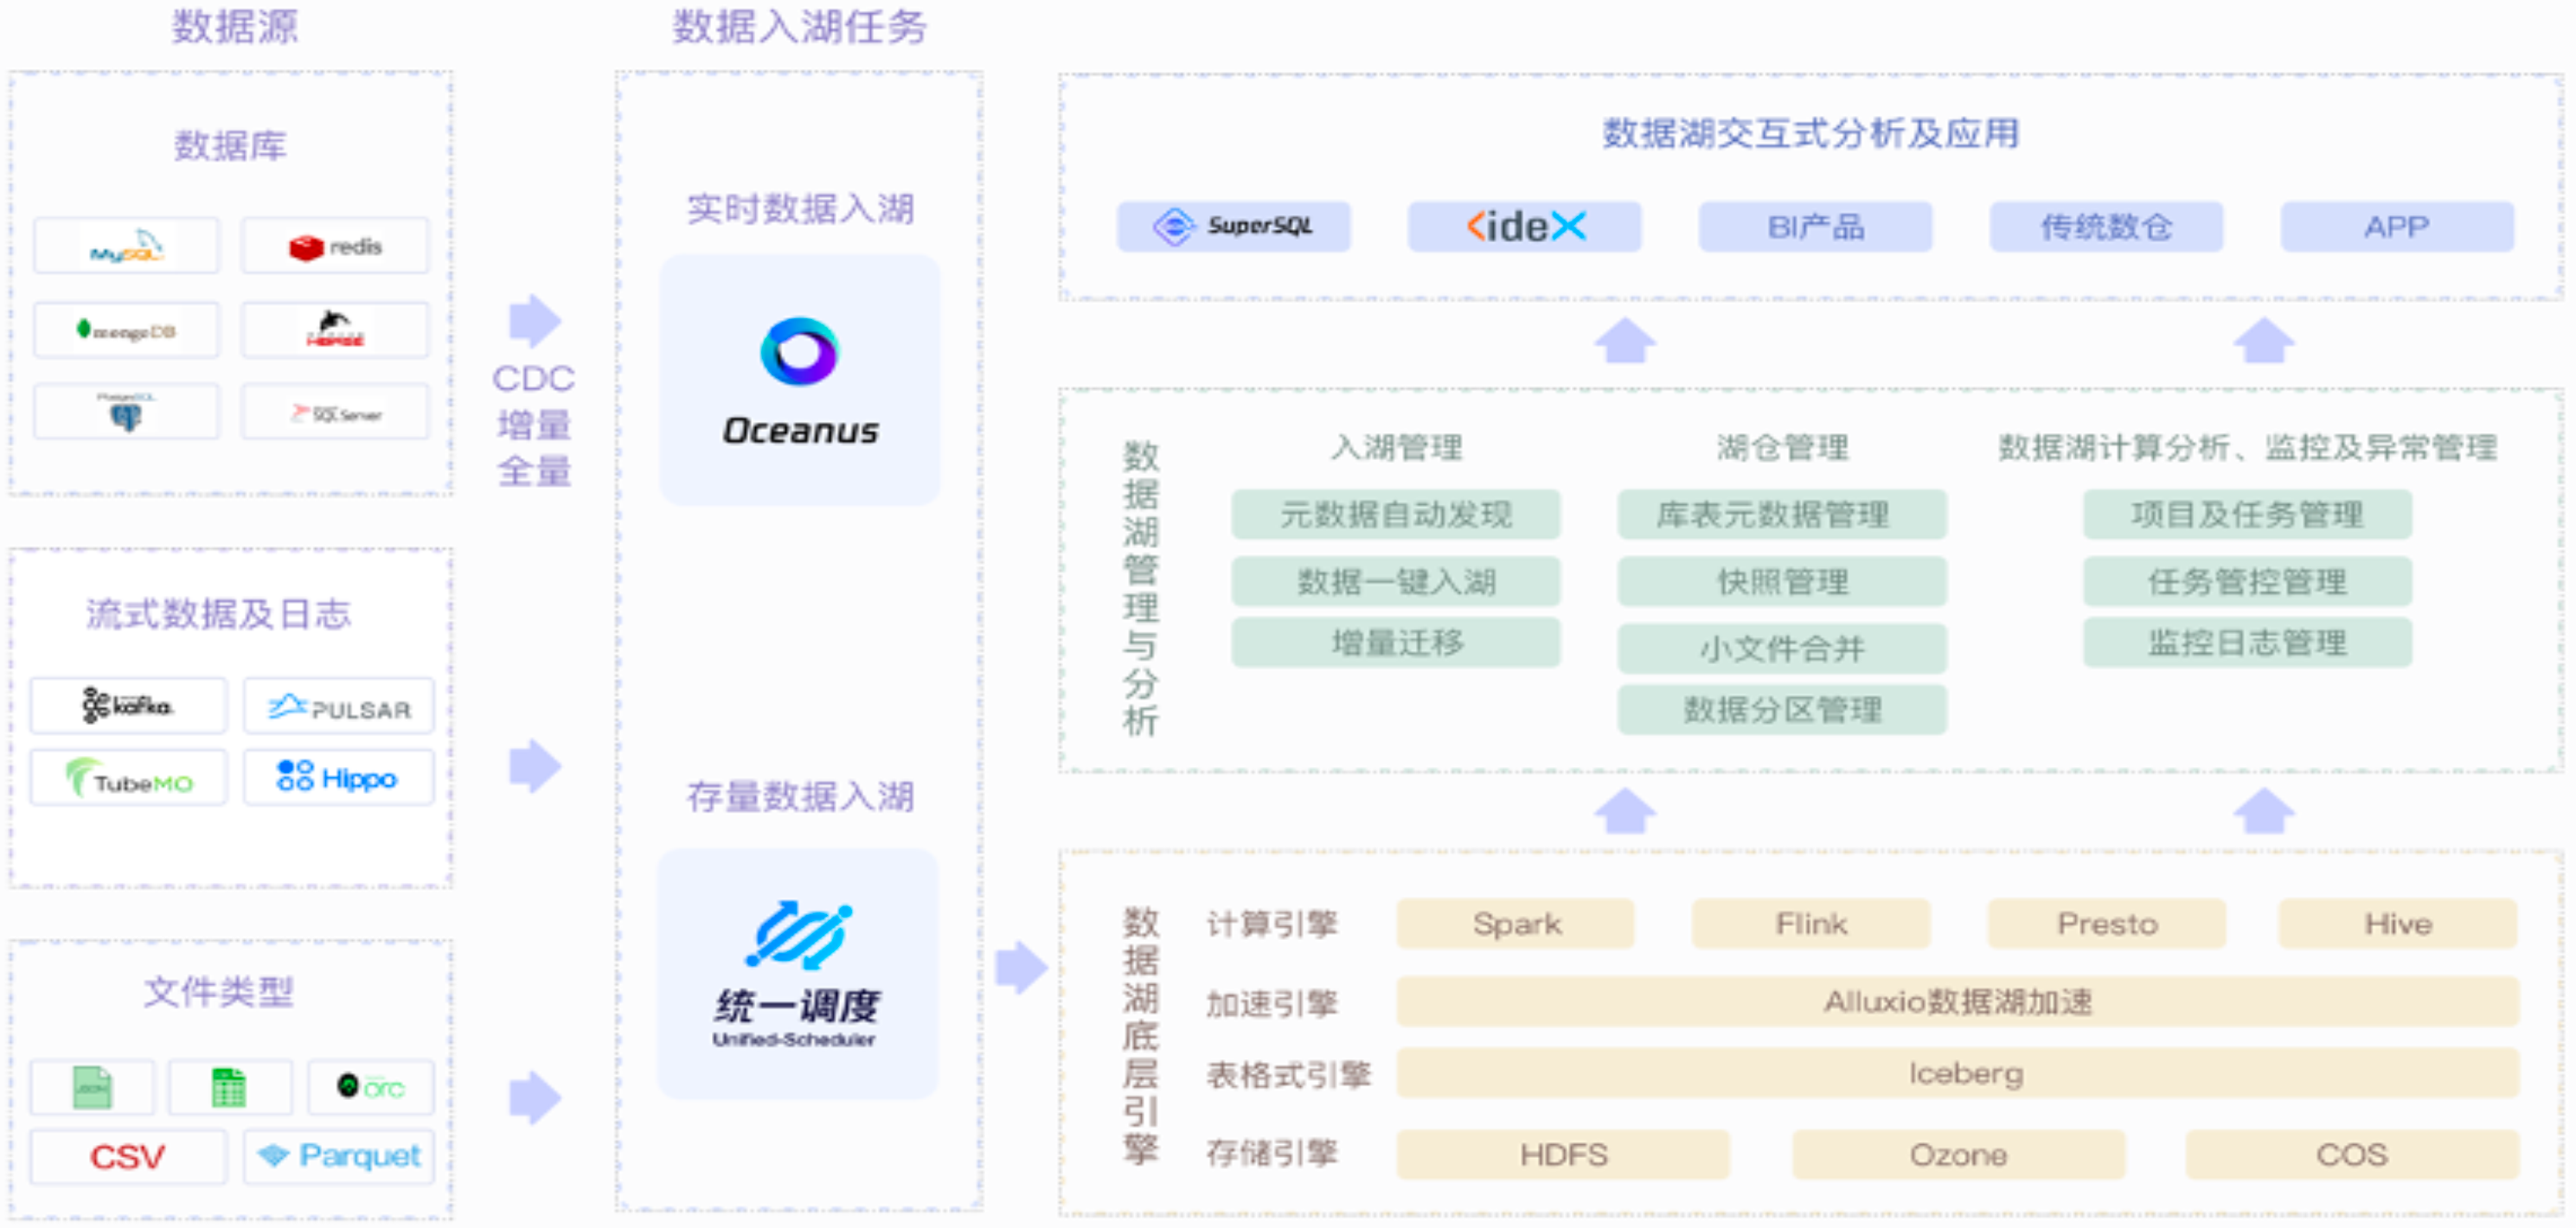
\includegraphics[width=1.0\textwidth]{功能架构图.png}
  \caption{功能架构图}
  \label{fig:功能架构图}
\end{figure}

\subsection{系统架构设计}

数据湖分析系统的主要系统架构如图\ref{fig:系统架构图}所示,用户通过浏览器的前端页面访问服务器,服务器根据收到的请求进行业务层操作,
业务层主要包括数据源管理、元数据管理、数据入湖、数据探索、自动优化五个功能,而业务层的操作需要相关权限的认证,
接着会将有用的信息进行数据持久化操作,系统的数据持久化能力主要由Mysql作为系统的数据库提供,系统运行的主机是腾讯云的主机,
三台8核16G的机器作为系统部署的机器。

\begin{figure}[H]
  \centering
  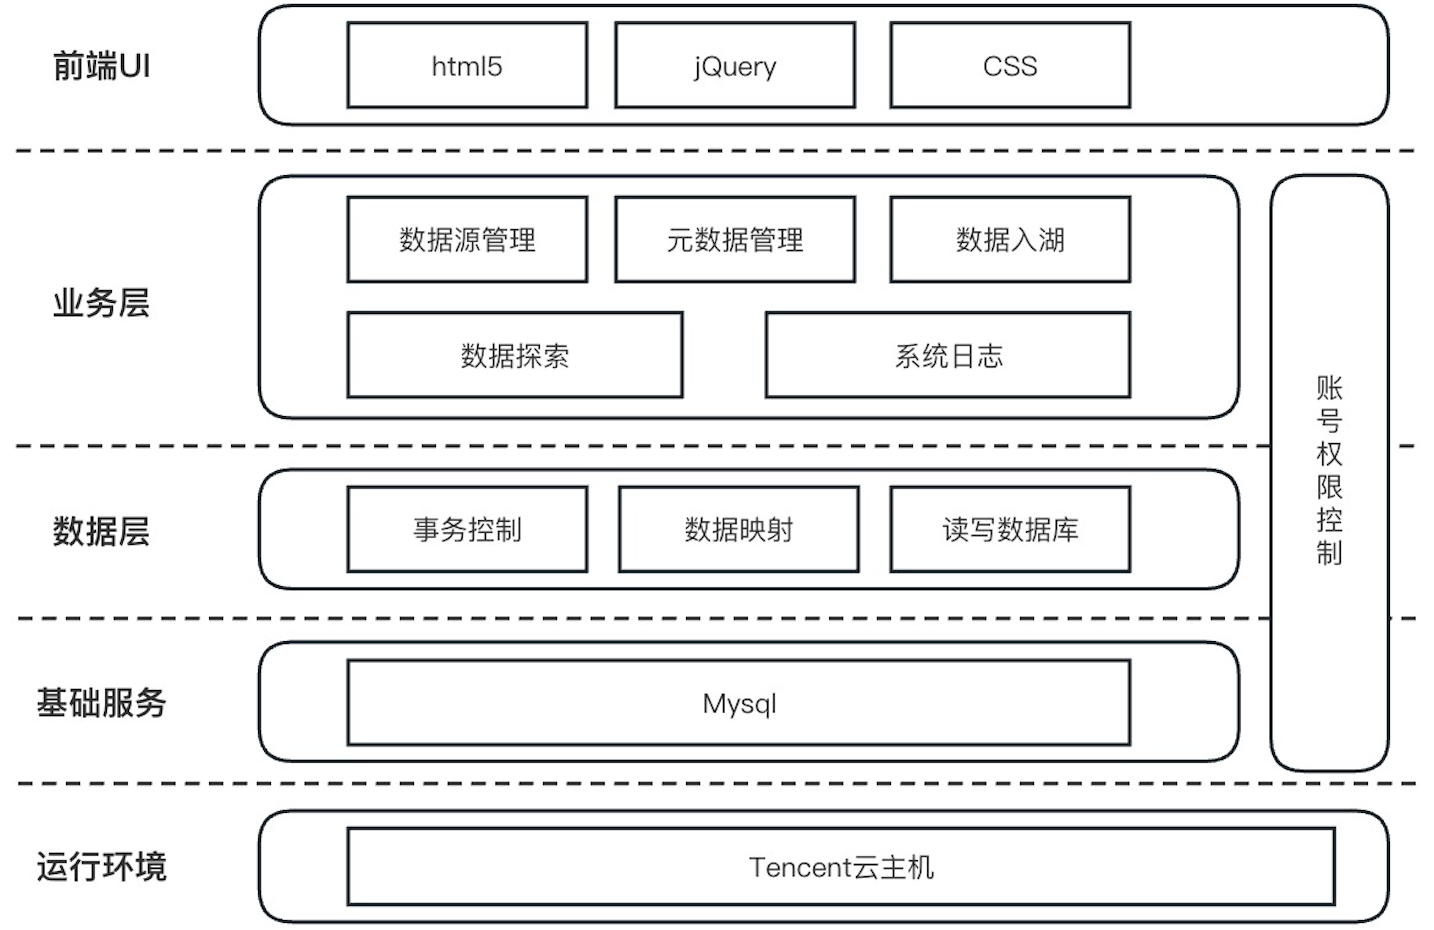
\includegraphics[width=1.0\textwidth]{系统架构图.png}
  \caption{系统架构图}
  \label{fig:系统架构图}
\end{figure}

\section{系统功能模块设计}

根据上一章对数据湖分析系统的需求分析,将系统划分了五个功能:数据源管理、元数据管理、数据入湖、数据探索、自动优化,
本节将对这五个功能模块进行概要设计。

\subsection{数据源管理}

数据源是入湖任务必须设置的,是Iceberg入湖的源头,该模块支持数据源创建、查看、编辑、删除功能。
在系统上创建数据源,需要填好所需要的信息,然后会做一个连接测试,最后才会将该数据源持久化到mysql中。
创建数据源的时序图如图\ref{fig:数据源创建时序图}所示:

\begin{figure}[H]
  \centering
  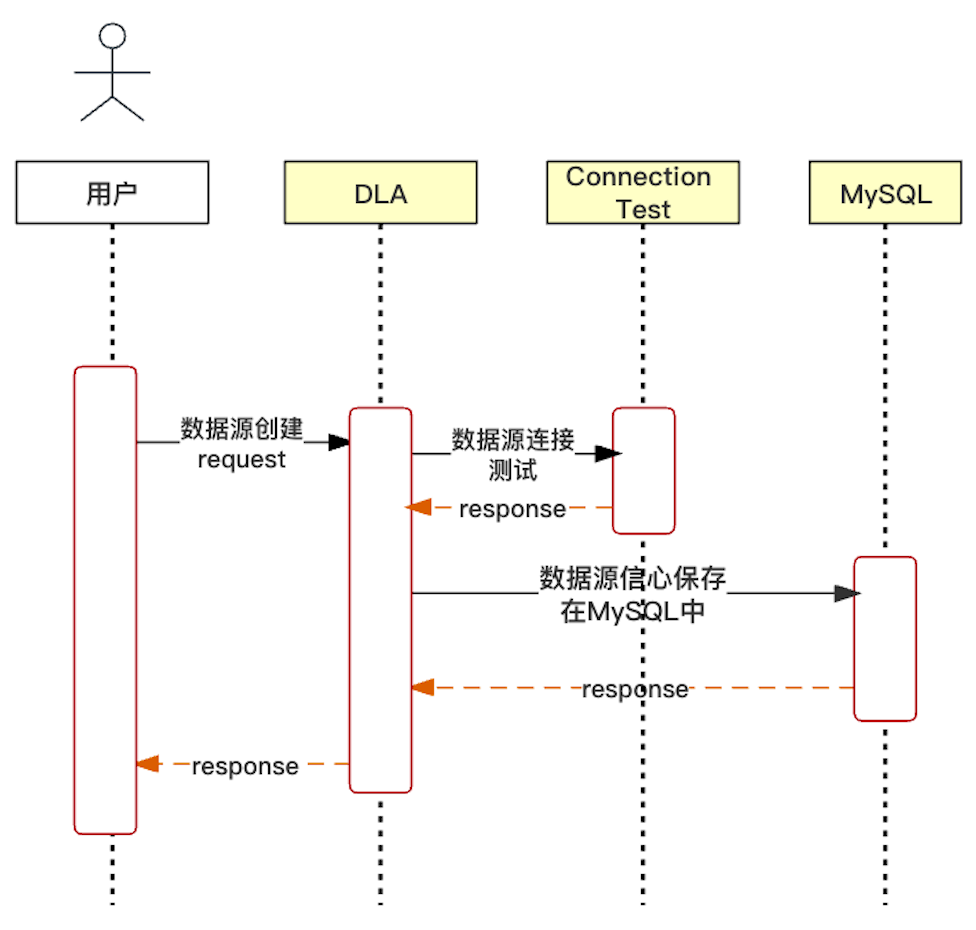
\includegraphics[width=1.0\textwidth]{数据源创建时序图.png}
  \caption{数据源创建时序图}
  \label{fig:数据源创建时序图}
\end{figure}

从数据源分类上来看,数据湖分析系统支持关系型数据库源
(mysql)以及消息队列数据源(tube、kafka、pulsar),各数据源需要的信息字段如下:

(1)创建mysql数据源需要的信息字段如表\ref{tab:mysql数据源需要的信息字段}所示:

\begin{table}[H]
  \centering
  \caption{mysql数据源需要的信息字段}
  \label{tab:mysql数据源需要的信息字段}
  \begin{tabular}{clcl}
    \toprule
    序号  & 字段名     & 是否空值   & 说明    \\
    \midrule
    1    & 数据源名称  & N        & 入湖任务通过mysql数据源名称  \\
         &           &          & (表名)指向mysql中的表      \\
    2    & 描述       & Y        & 对数据源的描述                                \\
    3    & 用户名     & N        & 与mysql用户名一致                             \\
    4    & 密码       & N        &  与mysql密码一致                             \\
    5    & 库名       & N        &   mysql中要入湖的数据库                       \\
    6    & 服务器地址  & N        &  可以是ip或者能解析的域名                      \\
    7    & 服务器端口  & N        &   mysql数据库端口号                          \\
    \bottomrule
  \end{tabular}
\end{table}

(2)创建tube数据源需要的信息字段如表\ref{tab:tube数据源需要的信息字段}所示:

\begin{table}[H]
  \centering
  \caption{tube数据源需要的信息字段}
  \label{tab:tube数据源需要的信息字段}
  \begin{tabular}{clcl}
    \toprule
    序号  & 字段名     & 是否空值   & 说明                                      \\
    \midrule
    1    & 数据源名称  & N        & 入湖任务通过TUBE数据源   \\
         &           &          & 名称指向tube中的表       \\
    2    & 描述       & Y        & 对数据源的描述                                \\
    3    & TUBE业务ID     & N        & TUBE业务ID名称                             \\
    4    & TUBE服务器列表       & N        &  系统填充,输入正确的TUBE业务     \\
         &                   &            &  ID后会自动填充对应的列表         \\
    \bottomrule
  \end{tabular}
\end{table}

(3)创建kafka数据源需要的信息字段如表\ref{tab:kafka数据源需要的信息字段}所示:

\begin{table}[H]
  \centering
  \caption{kafka数据源需要的信息字段}
  \label{tab:kafka数据源需要的信息字段}
  \begin{tabular}{clcl}
    \toprule
    序号  & 字段名     & 是否空值   & 说明                                      \\
    \midrule
    1    & 数据源名称  & N        & 入湖任务通过kafka服务器  \\
         &           &          &  地址指向kafka中的表 \\
    2    & 描述       & Y        & 对数据源的描述                               \\
    3    & Kafka服务地址    & N        & kafka服务地址                           \\
    4    & Kafka版本号      & N        &  kafka版本号       \\
    \bottomrule
  \end{tabular}
\end{table}

(4)创建Pulsar数据源需要的信息字段如表\ref{tab:Pulsar数据源需要的信息字段}所示:

\begin{table}[H]
  \centering
  \caption{Pulsar数据源需要的信息字段}
  \label{tab:Pulsar数据源需要的信息字段}
  \begin{tabular}{clcl}
    \toprule
    序号  & 字段名     & 是否空值   & 说明                                      \\
    \midrule
    1    & 数据源名称  & N        & 入湖任务通过Pulsar服务器 \\
         &           &          &  地址指向Pulsar中的表 \\
    2    & 描述       & Y        & 对数据源的描述                               \\
    3    & Pulsar业务ID    & N        & Pulsar业务ID                          \\
    4    & Pulsar服务地址      & N        &  系统填充,输入正确的Pulsar业务   \\
         &                    &         &  ID后会自动填充对应的服务地址      \\
    \bottomrule
  \end{tabular}
\end{table}

\subsection{元数据管理}

元数据管理是用来管理iceberg表元数据的,包含四个主要的功能,分别是数据自动优化,表的创建、编辑、查看、删除,关联已创建的表,库操作。
因为自动优化会修改元数据,所以自动优化是属于元数据管理的,在后面的小节会进行详细介绍。

其中表的创建需要和安全中心、hive metastore、mysql进行交互,
创建Iceberg表的时序图如图\ref{fig:创建Iceberg表时序图}所示,可以看到一个createTable的request建立后,
首先到安全中心判断用户是否有该数据库的create table权限,有才能进行下一步,
接着会判断metastore中是否已存在表,若不存在,则会判断MySQL中是否存在对应的DB和table,
这里MySQL中的DB和table实质上是一个映射,是用来方便在系统页面展示表元数据的,若MySQL中不存在,
则创建对应的DB和table,接着会在metastore中创建实际的iceberg表元数据;表的查看直接去
MySQL中查看即可;表的编辑如果涉及到字段的增加及删除操作,则会更新metastore中对应的
表元数据;若已在其它平台创建了iceberg表,则可通过metastore的元数据进行关联;
库操作包括注册和查看,其中注册需要进行申请,需要安全中心相关负责人审批后才能注册成功。

\begin{figure}[H]
  \centering
  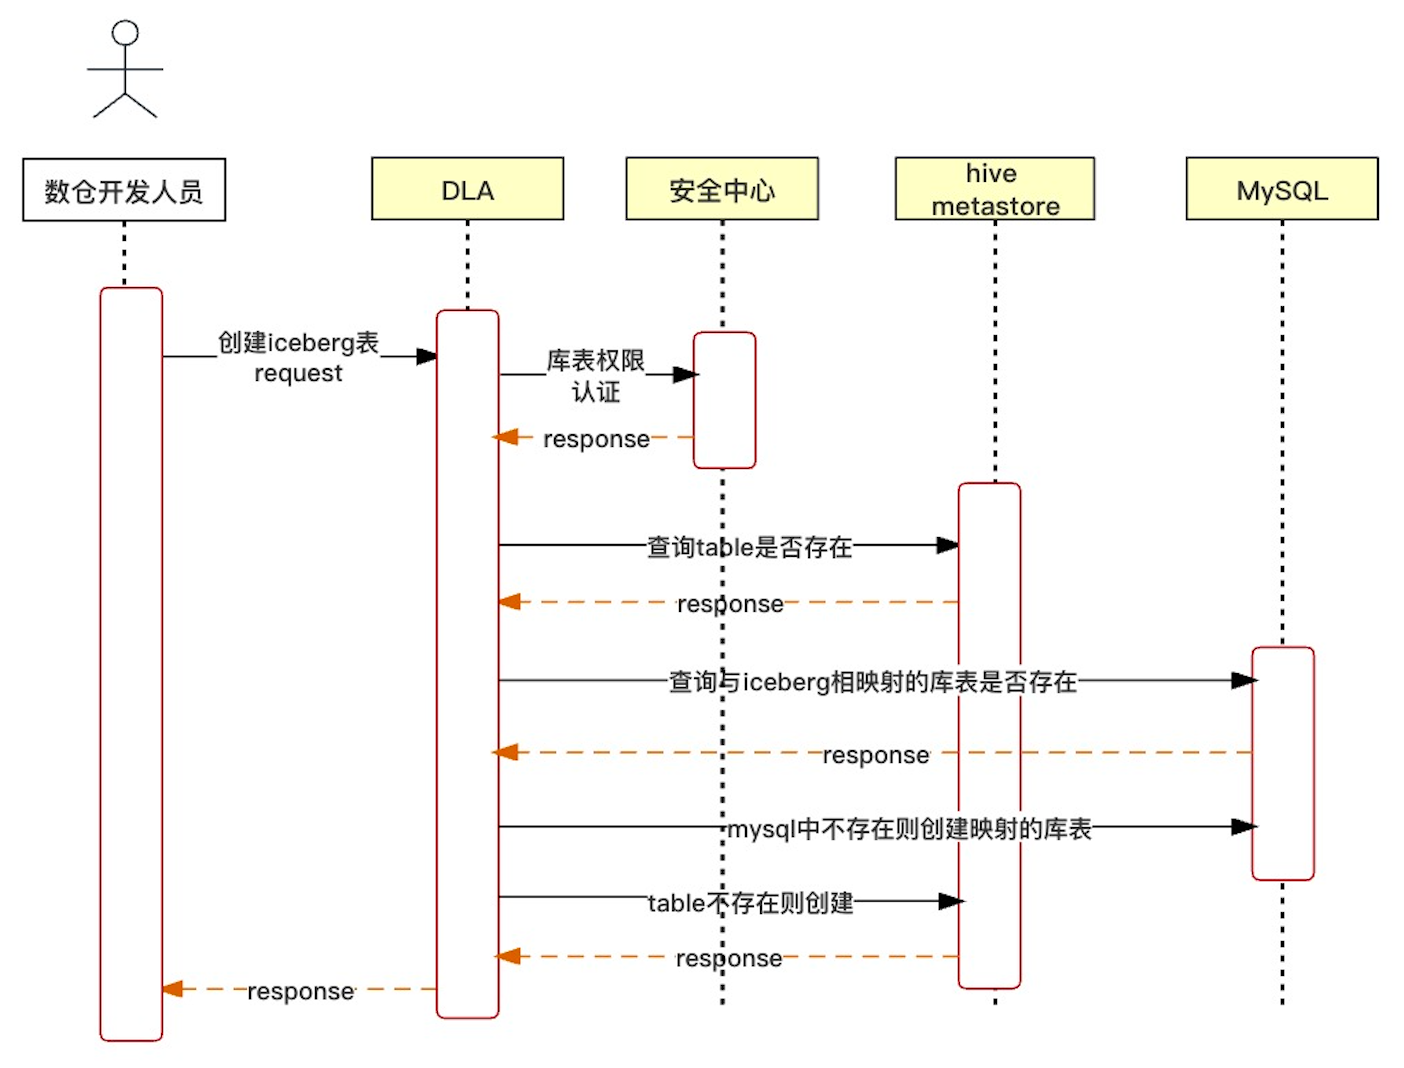
\includegraphics[width=1.0\textwidth]{DLA创建Iceberg表时序图.png}
  \caption{创建Iceberg表时序图}
  \label{fig:创建Iceberg表时序图}
\end{figure}

\subsection{数据入湖}

数据入湖是数据湖分析系统的核心流程功能,目的是用户通过该功能将源数据表流程化入湖
和查看已申请入湖任务执行情况。入湖任务分为三类,分别为实时数据入湖、存量数据入湖
和关系型数据入湖,三类入湖任务的创建都需要填写基础信息、源表、目标表、参数及资源,
若目标表在任务创建的时候还没有创建,则会自动的根据填写的字段信息生产对应的目标表,
即在对应的数据库中生成iceberg表,因为需要访问元数据,所以也会在安全中心进行权限认证。
入湖任务创建的时序图如图\ref{fig:入湖任务创建时序图}所示。

入湖任务都会生成对应的jar包,若为实时数据入湖,则会在公司内部的实时流计算平台
Oceanus上创建对应的jar任务,底层使用的引擎是flink;若为存量数据入湖或者关系
型数据入湖,则会在定时任务执行平台US上创建jar任务,底层使用的引擎是spark,
并可在系统页面上设置任务执行的时间间隔和起始时间。

\begin{figure}[H]
  \centering
  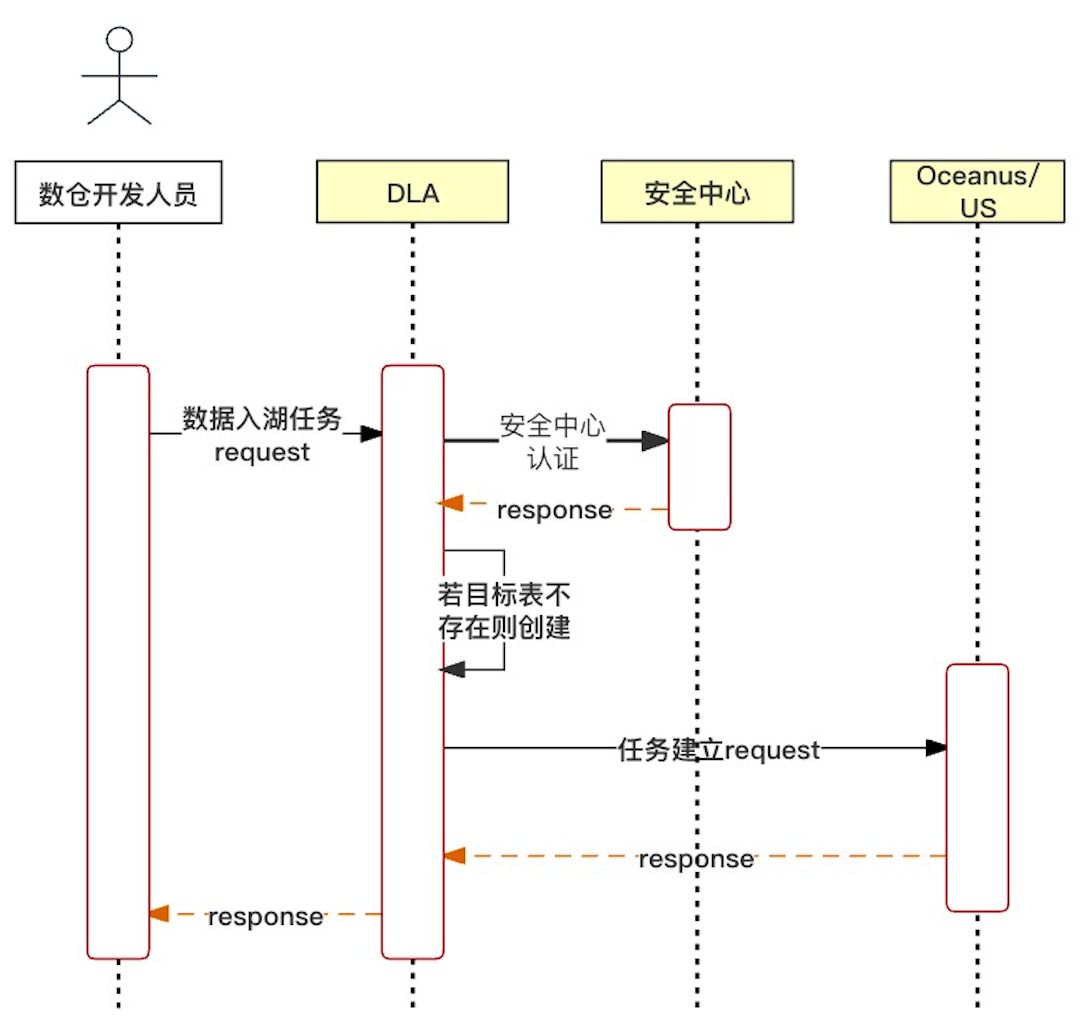
\includegraphics[width=0.9\textwidth]{入湖任务创建时序图.png}
  \caption{入湖任务创建时序图}
  \label{fig:入湖任务创建时序图}
\end{figure}

\subsection{数据探索}

数据探索功能是数据入湖后,用户需要进行数据查看或者数据分析时使用的工具,
目前主要依赖内部统一查询平台实现数据探索功能,在该平台上,用户可以编写sql
设置执行引擎,presto或者spark。其中presto查询速度快,但是功能少,
只支持查询功能;spark虽然查询速度慢,但支持的语句功能比较多,支持创建表、
删除表、更新表、数据写入、数据删除、更新分区、表维护等语句。在查询平台上的数据探索时序图如图\ref{fig:数据探索时序图}所示。

\begin{figure}[H]
  \centering
  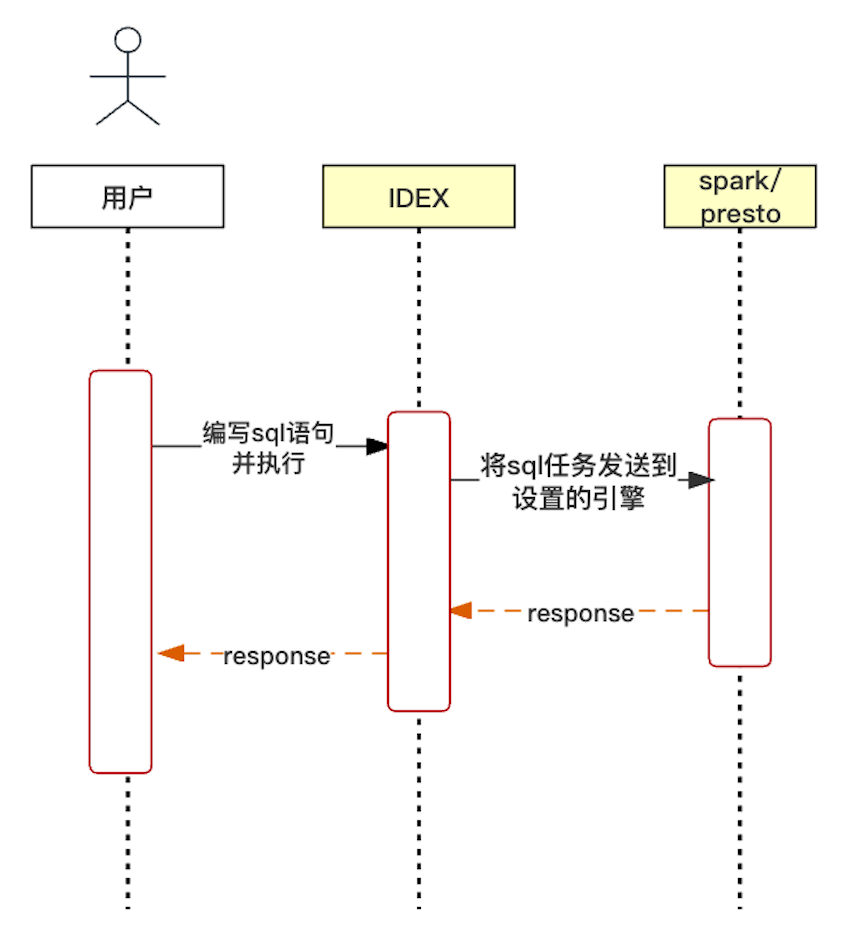
\includegraphics[width=0.7\textwidth]{数据探索时序图.png}
  \caption{数据探索时序图}
  \label{fig:数据探索时序图}
\end{figure}

除了统一查询平台可以进行数据探索外,DLA还提供了Zeppelin进行数据探索,Zeppelin是一个基于Web的notebook,
可以进行数据探索和可视化。它可以接入多种数据处理引擎,如spark、hive等,并支持多种语言,
如Scala、Python、SparkSQL、Hive、Markdown、Shell等。开发者还可以实现更多的解释器来添加数据引擎。

\subsection{自动优化服务}

Iceberg是基于快照的表格式,当两次commit间隔的数据量较小的情况下就会产生小文件,
这种案例在iceberg被做为flink sink(流式场景)时尤为常见。用户为了下游引擎能高效的查询iceberg,
经常会构建一些辅助的数据优化任务去优化iceberg表,例如、小文件合并、快照历史清理、孤儿文件删除。
为了让用户能更方便的使用iceberg表,优化总体基于iceberg表数据湖的成本和性能,
这里提出数据智能运维的概念,通过平台提供的统一服务对iceberg表进行优化从而降低整体数据湖的成本和性能的优化。

\begin{figure}[H]
  \centering
  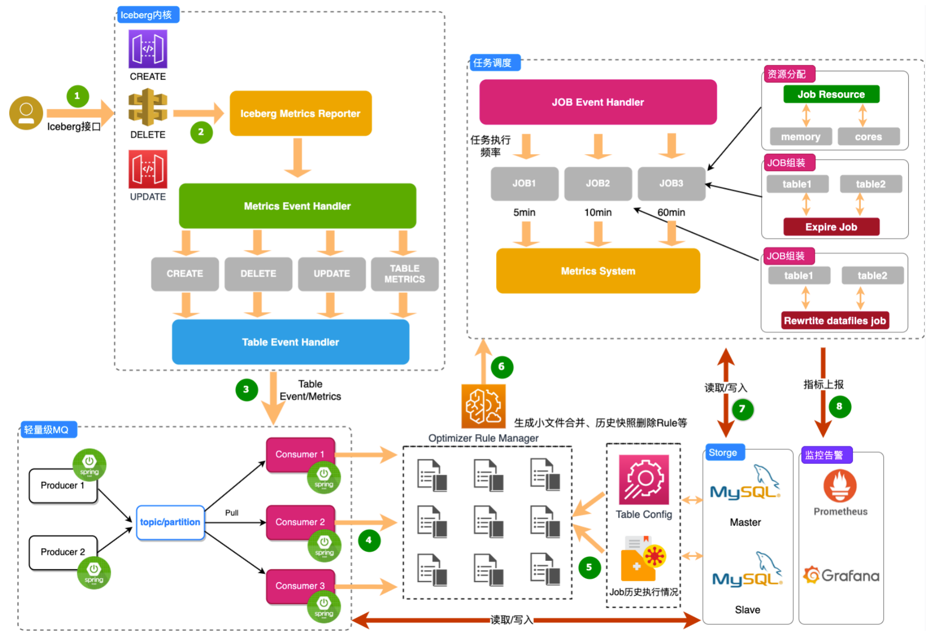
\includegraphics[width=1.0\textwidth]{自动优化总体流程图.png}
  \caption{自动优化总体运行流程图}
  \label{fig:自动优化总体运行流程图}
\end{figure}

自动优化服务的总体运行流程图如图\ref{fig:自动优化总体运行流程图}所示,可以看到整个服务中的数据流。
先简单介绍小文件合并服务,当用户对Iceberg进行操作时,自动优化服务已经为Iceberg
实现了汇报Metrics到外部系统的功能。Metrics的Reporter会将Iceberg的建表、
删除、更新或Commit操作产生的snapshot的summary报告到Iceberg的Metrics事件
处理程序。Metrics事件处理程序会根据不同事件的类型将这些事件存储到MySQL中。这里
自动优化服务改进了这个过程,采用了消息队列来确保事件的时效性,并且定期将消息队列中的数据保存在MySQL中。
表的一些基本的记录信息,如表在合并前后的文件数量、操作类型等Metrics信息。
在数据通过消息队列发送到中间阶段时,规则管理器会根据用户配置的规则配置大量规则。
例如,一些用户希望在每产生100个10M文件时对表进行一次合并。这些规则接口开放给
用户配置,配置传递给下游任务调度器。任务读取器读取上游发送的规则,以决定根据这些规则启动什么样的任务。
图中可以看到下游有许多不同的任务,如JOB1、JOB2、JOB3。为处理上游发送的信息,自动优化服务目前使用离线的Spark任务。
任务执行频率根据用户配置的表而定,可以是5分钟、10分钟、60分钟等。如果用户表需要保留过去100个文件,
而用户提交频率很高,可能在单位时间内产生大量文件,那么就需要以5分钟为单位执行一次合并文件操作。对于提交频率
较低的用户,可以以小时级别或每5个小时执行一次文件处理调度任务,根据不同用户表的一些metrics情况决
定将用户表放在哪个粒度的调度任务中执行。
目前,每个job可以处理多个用户的表,每次处理完后,将这些表的处理结果通过Metrics System消息队列
反馈给MySQL记录。然后通过Grafana或其他监控工具可以查看任务的运行情况,包括合并后表的状态等。
此外,还记录每次合并文件任务的执行时间,以便通过Job Handler动态地调整每个job所处理的表的数量。
例如,如果一个job处理1、2、3三个表,发现表1和表2执行的合并任务只花费10秒钟,而表3花了5分钟,
由于任务是串行提交的,因此必须等到第三个表执行完毕后,才能继续调度下一次任务。
那么自动优化服务可以在下次调度时将表3调度到其他任务区,让表1和表2在一分钟内不断处理文件合并。

\subsubsection{合并小文件}

由于原有的Iceberg小文件合并方式在实际应用中存在很多问题,
如合并不及时、浪费资源以及占用计算资源过多等,因此重新设计了小文件合并规则。

由于合并的任务无法知道当前的文件状态,因此需要一种计算规则来判断当前一个区间内
是否达到了发起合并任务的时刻,即需要计算出文件的状态,以作为合并任务调度的合并规则。这里自动优化服务采用的是均方误差(MSE)的计算方法。

均方误差的数学含义是表示一个样本区间内样本值与目标值之间差异程度的一种度量,
假如设定合并后大文件的目标大小为512MB,则这个样本区间就是512MB,如果MSE的值越大,
表示当前样本区间内的文件相对于目标大小的差值也越大,因此可以设定一个阈值来决定合并的粒度,
例如设置一个阈值T,当阈值T越大表示合并的区间内小文件的比例要越高才会被触发到合并。如图\ref{fig:小文件合并触发示意图}所示,
分区0中三个文件大小相对于目标文件大小相差很大,导致该分区MSE值大于阈值T,将会进行合并,而分区1中三个文件的大小和目标文件的大小
差不多,该分区的MSE小于阈值T,将不会进行合并。

\begin{figure}[H]
  \centering
  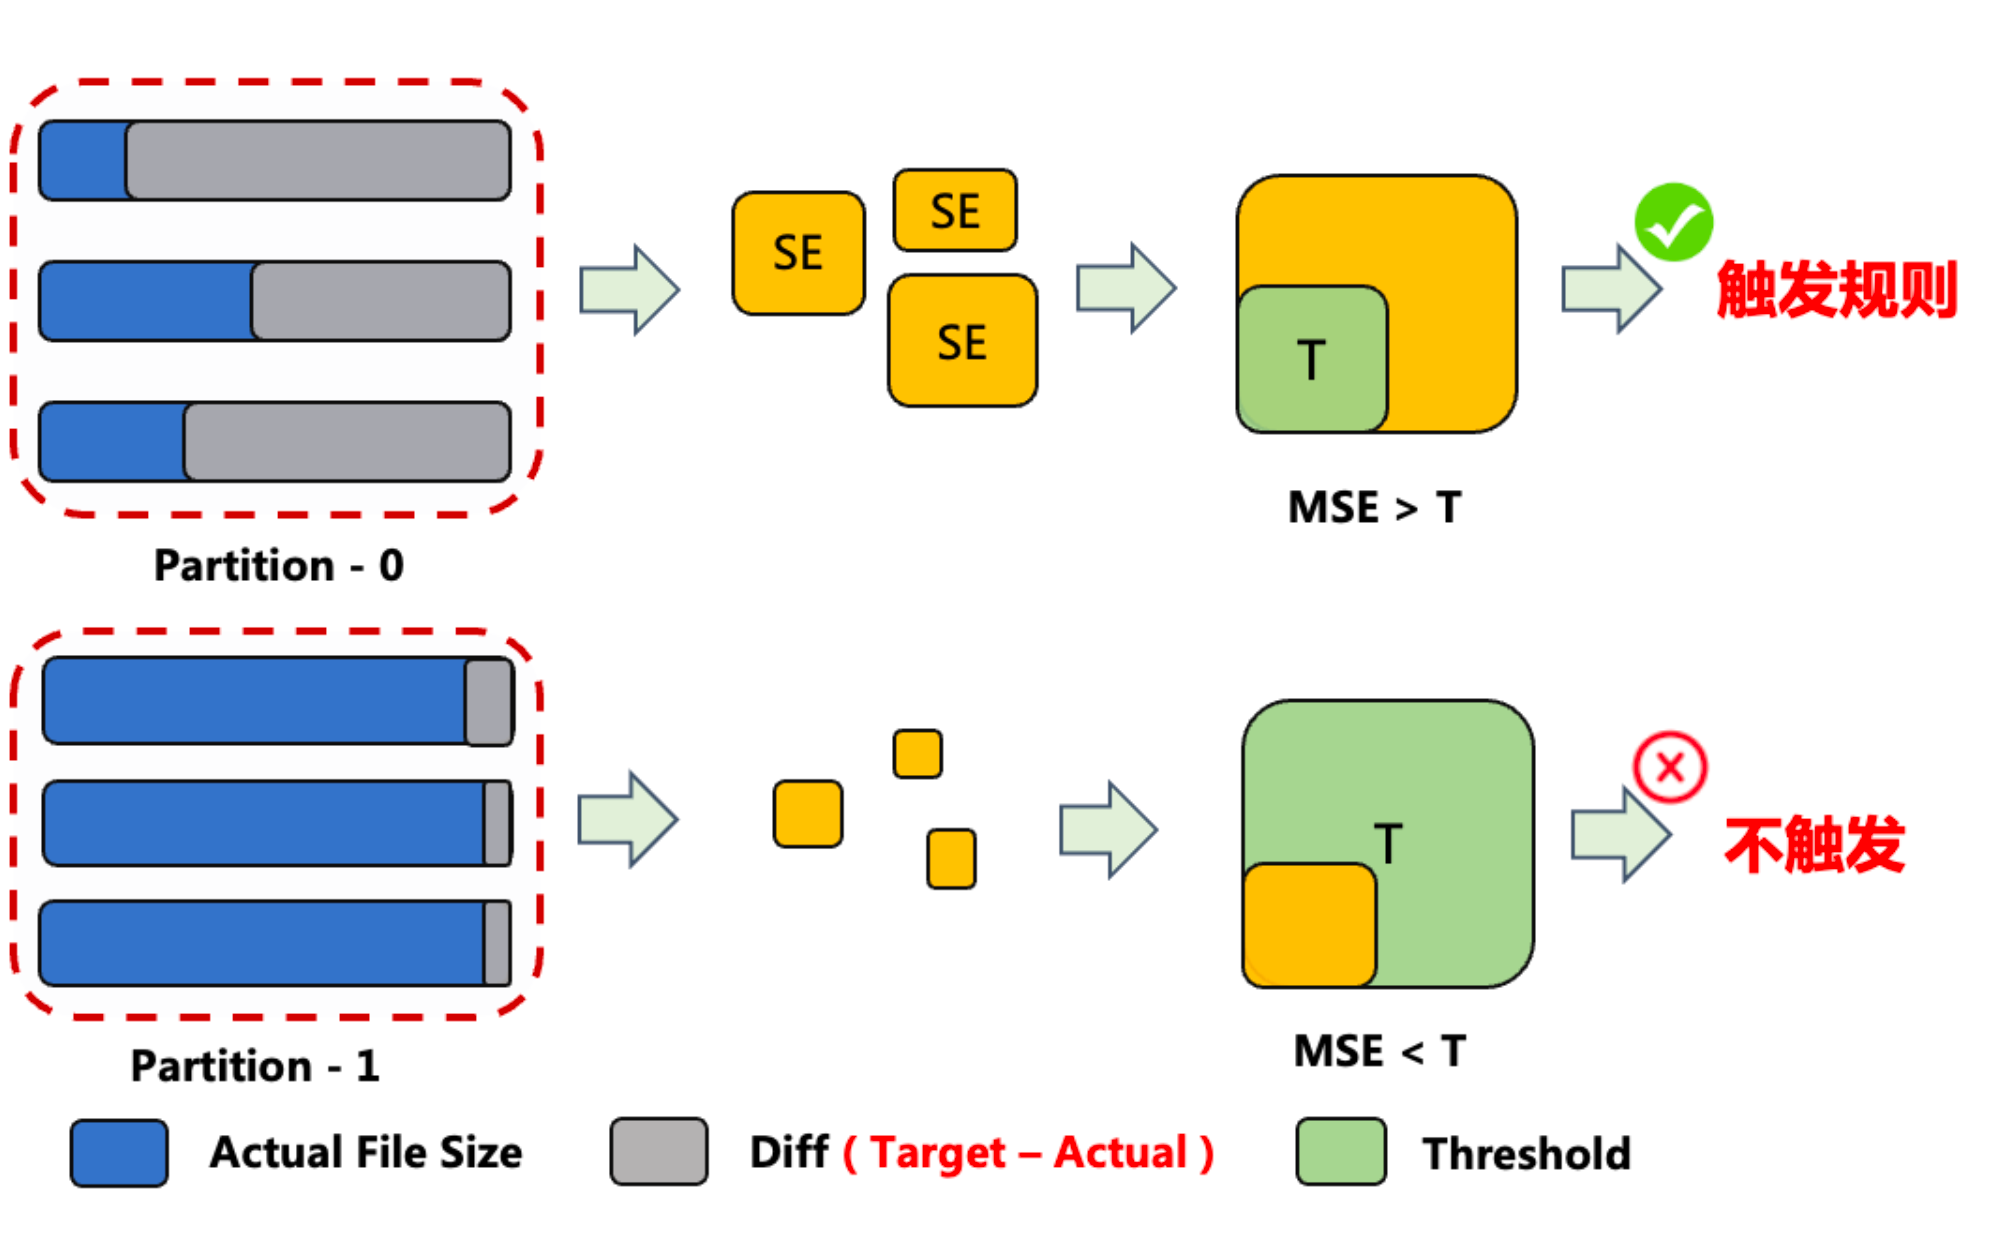
\includegraphics[width=1.0\textwidth]{小文件合并触发示意图.png}
  \caption{小文件合并触发示意图}
  \label{fig:小文件合并触发示意图}
\end{figure}

\subsubsection{历史快照清理}

Iceberg表每一次write都会产生一个新的snapshot,同时也会产生一个新的version版本。
所以对于流式写入,会产生大量的snapshot。
对于历史快照的清理,需要配置两个参数,快照失效时间和快照保留数量,
其中所配置的快照失效时间以小时为粒度,快照删除的触发条件如图\ref{fig:历史快照删除触发条件}所示,
超过所设置的时间或者超过了快照保留的阈值快照将被删除。

\begin{figure}[H]
  \centering
  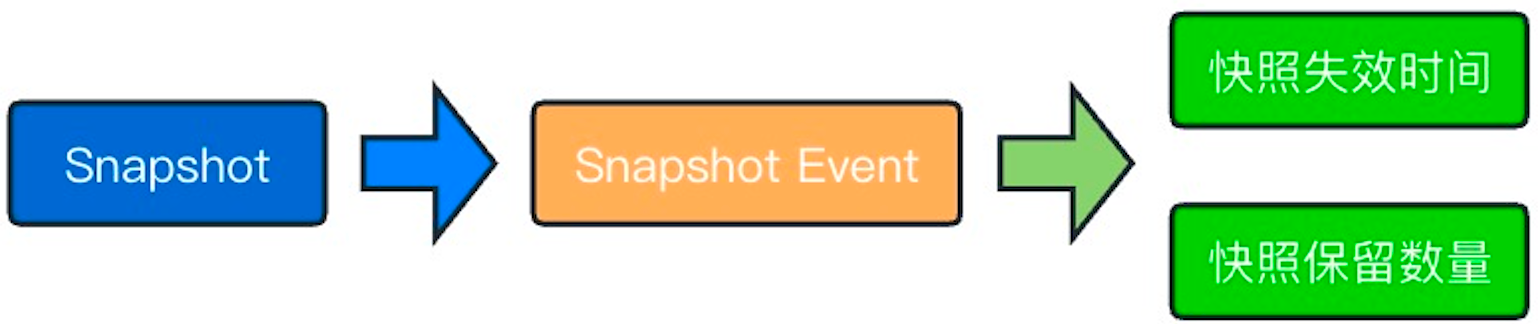
\includegraphics[width=1.0\textwidth]{历史快照删除触发条件.png}
  \caption{历史快照删除触发条件}
  \label{fig:历史快照删除触发条件}
\end{figure}

\subsubsection{孤儿文件删除}

对于那些没有被引用的孤儿文件的删除,有以下注意事项:

(1)可能表下面有许多data和metadata files需要被删除,会花费大量的时间,所以不要频繁进行孤立文件的删除;

(2)有时一个write操作可能会花费很长的时间,比如一天。在这期间就会产生很多被认为是孤立的文件。
所以孤立文件的保留时间要大于write的时间,默认是3天

(3)在一些文件系统,一份文件的路径相关属性发生改变,就会被误认为是孤立文件而被删除。
例如在HDFS中,将一个data file的权限进行修改,该data file可能不能和其他metadata file进行关联,就被误认为是孤立文件而被删除。

综合上面的考虑,需要设置一个孤儿文件过期时间,用来定时的扫描文件进行孤儿文件的清除,过期时间默认为3天。

\subsubsection{数据生命周期管理}

⽣命周期管理是对表级别中的数据起作用的,需要schema中有Date或TimeStamp类型的时间字段,并且需要用户设置一个expireTime。
若对该表启动了⽣命周期管理并指定了时间列,然后底层根据所设置的expireTime进⾏数据删除。
通过生命周期管理,用户可以方便地控制不再需要的数据的自动删除,从而释放存储空间和资源。
但这样的⽣命周期管理有一些限制:

(1)⽬前仅⽀持long(10/13位)、date、timestamp等类型时间字段;

(2)expireTime根据dataFile中的upperbounds值进⾏筛选,如果upperBound值为null将⽆效。

\section{系统数据库设计}

在信息存储方面,数据湖分析系统主要使用mysql进行信息存储,主要包括任务信息、任务详情信息、
目标库信息、目标表信息、数据源信息、任务jar包信息,其中目标库和目标表在mysql
中的信息只是一个映射,具体实际的表还是Iceberg表,其元数据存放在hive metastore中,
数据文件存储在HDFS集群上。数据库ER图如图\ref{fig:数据库ER图}所示,任务表和
目标表、数据源表、任务详情表、任务jar包信息表都是1对1的关系,而目标库和目标表的关系是1对多的关系,
表示一个数据库中可以有多张iceberg表。

\begin{figure}[H]
  \centering
  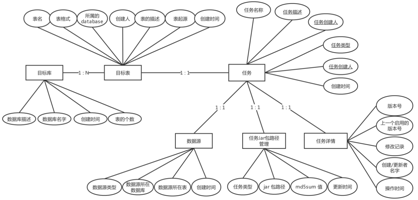
\includegraphics[width=1.0\textwidth]{数据库ER图.png}
  \caption{数据库ER图}
  \label{fig:数据库ER图}
\end{figure}

系统中主要的数据库表格结构设计如下:

(1)任务表(dlaTask)详细描述如表\ref{tab:任务表}所示。

\begin{table}[H]
  \centering
  \caption{任务表}
  \label{tab:任务表}
  \begin{tabular}{clllcl}
    \toprule
    序号  & 字段名         & 字段说明     & 类型           & 是否可为空   & 说明  \\
    \midrule
    1    & id            & 任务id      & bigint(20)     & N          & PRIMARY KEY    \\
    2    & name          & 任务名称     & varchar(256)   & N          &     \\
    3    & desc          & 任务描述     & text           & Y          &   \\
    4    & tableId       & 目标表id     & bigint(20)     & N          &   \\
    5    & type          & 任务类型     & tinyint(4)     & N          & 1-Oceanus实时  \\
         &               &             &               &             & 2-US存量  \\
    6    & actualTaskId  & 实际的任务id  & bigint(20)    & N          &  1-Oceanus任务id  \\
         &               &             &               &             & 2-US任务id  \\
    7    & creatorName   & 创建者       & varchar(64)    & N          &   \\
    8    & createTime    & 创建时间     & timestamp      & N          &   \\
    9    & deleted       & 是否被删除    & boolean        & N          &   \\
    10   & numRetries    & 重试次数      & int(4)        & N          &   \\
    \bottomrule
  \end{tabular}
\end{table}

(2)任务详情表(dlaTaskDetail)详细描述如表\ref{tab:任务详情表}所示。

\begin{table}[H]
  \centering
  \caption{任务详情表}
  \label{tab:任务详情表}
  \begin{tabular}{clllcl}
    \toprule
    序号  & 字段名              & 字段说明     & 类型           & 是否可为空   & 说明  \\
    \midrule
    1    & id                 & 任务详情id   & bigint(20)     & N          & PRIMARY KEY    \\
    2    & taskId             & 任务id      & bigint(20)     & N          &    \\
    3    & version            & 任务版本     & bigint(10)     & N          &   \\
    4    & lastEffectVersion  & 上一个版本   & bigint(10)     & N          &   \\
    5    & modification       & 修改记录     & text           & Y          &   \\
    6    & updateUser         & 更新者       & varchar(64)   & N          &    \\
    7    & updateTime         & 操作时间     & timestamp      & N          &   \\
    8    & taskDetail         & 任务详情     & text           & N          &   \\
    \bottomrule
  \end{tabular}
\end{table}

(3)目标库(dlaDatabase)详细描述如表\ref{tab:目标库}所示。

\begin{table}[H]
  \centering
  \caption{目标库}
  \label{tab:目标库}
  \begin{tabular}{clllcl}
    \toprule
    序号  & 字段名              & 字段说明     & 类型           & 是否可为空   & 说明  \\
    \midrule
    1    & id                 & 目标库id     & bigint(20)    & N          & PRIMARY KEY    \\
    2    & name               & 数据库名称    & varchar(256)  & N          &    \\
    3    & desc               & 数据库描述    & text          & Y          &   \\
    4    & tableNum           & 表的个数      & Int           & N          &   \\
    5    & createTime         & 创建时间      & timestamp     & N          &   \\
    \bottomrule
  \end{tabular}
\end{table}

(4)目标表(dlaTable)详细描述如表\ref{tab:目标表}所示。

\begin{table}[H]
  \centering
  \caption{目标表}
  \label{tab:目标表}
  \begin{tabular}{clllcl}
    \toprule
    序号  & 字段名              & 字段说明     & 类型           & 是否可为空   & 说明  \\
    \midrule
    1    & id                 & 目标表id     & bigint(20)    & N          & PRIMARY KEY    \\
    2    & name               & 表名         & varchar(256)  & N          &    \\
    3    & format             & 表格式       & tinyint(4)    & N          & 1-iceberg  \\
    4    & dbName             & 所属DB       & varchar(256)  & N          &   \\
    5    & creatorName        & 创建人       & varchar(64)   & N          &   \\
    6    & desc               & 表的描述     & text           & Y          &   \\
    7    & origin             & 表起源       & tinyint(4)    & N          & 1-数据湖页面创建的表   \\
         &                    &             &               &            & 2-其他地方同步  \\
    8   & createTime         & 创建时间     & timestamp     & N          &    \\
    \bottomrule
  \end{tabular}
\end{table}

(5)数据源表(dlaDatasource)详细描述如表\ref{tab:数据源表}所示。

\begin{table}[H]
  \centering
  \caption{数据源表}
  \label{tab:数据源表}
  \begin{tabular}{clllcl}
    \toprule
    序号  & 字段名              & 字段说明           & 类型           & 是否可为空   & 说明  \\
    \midrule
    1    & id                 & 数据源id           & bigint(20)    & N          & PRIMARY KEY    \\
    2    & type               & 数据源类型          & smallint(8)   & N          & 1-Tube   \\
         &                    &                   &               &            & 2-Kafka  \\
         &                    &                   &               &            & 3-Pulsar  \\
         &                    &                   &               &            & 4-Mysql  \\
    3    & actualTableId      & 所对应的真实tableId  & bigint(20)   & N          &   \\
    4    & sourceDB           & 所在数据库          & varchar(256)  & N          &   \\
    5    & sourceTable        & 所在表             & varchar(256)  & N          &   \\
    6    & createTime         & 创建时间           & timestamp     & N          &    \\
    \bottomrule
  \end{tabular}
\end{table}

(6)任务jar包管理表(dlaTaskJar)详细描述如表\ref{tab:任务jar包管理表}所示。

\begin{table}[H]
  \centering
  \caption{任务jar包管理表}
  \label{tab:任务jar包管理表}
  \begin{tabular}{clllcl}
    \toprule
    序号  & 字段名              & 字段说明           & 类型           & 是否可为空   & 说明  \\
    \midrule
    1    & id                 & 任务jar id        & bigint(20)     & N          & PRIMARY KEY    \\
    2    & type               & 任务类型           & tinyint(4)    & N           & 1-Oceanus实时   \\
         &                    &                   &               &            & 2-US存量   \\
    3    & jarPath            & jar包路径         & varchar(512)   & N          &   \\
    4    & md5sum             & md5sum校验值      & varchar(128)   & N          &   \\
    5    & updateTime         & 更新时间           & timestamp     & N          &   \\
    \bottomrule
  \end{tabular}
\end{table}

\section{本章小结}

本章主要阐述了数据湖分析系统的概要设计。首先介绍系统的总体架构,对
功能架构和系统架构进行了简单描述。另外根据上一章的需求分析,对系统的功能模块进行划分,并且详
细介绍了每个模块的功能设计。最后介绍了整个系统的数据库设计,展示数据库ER图以及主要的数据库表结构。

